\documentclass{article}

\input{natbib_article_preamble}

\begin{document}

\title{Random Matrix Theory}
\author{Alex Papanicolaou}
\date{\today}
\maketitle

\newcommand{\Tr}{\mathrm{Tr}}

I demonstrate here the fundamentals of RMT, the Marchenko-Pastur theorem, and
non-linear shrinkage, especially as it relates to minimizing out-of-sample
portfolio variance.  I will then try to sketch out how these results may be
extended to producing unbiased variance forecasts.

\section{Setup}

To begin, assume we observe i.i.d.\ random values in a $T \times N$ matrix,
$$
	X_N = \begin{bmatrix} 
					\text{---} & x_1    & \text{---} \\
					           & \vdots &            \\
					\text{---} & x_T    & \text{---}
				\end{bmatrix}
$$
where $T$ is the number of observations and $N$ is the number of variables (ie.
$x_i \in \mathbb{R}^N$).  I index by $N$ since $T$ and $N$ will be growing to
infinity.  In particular, we will take $T / N \rightarrow y > 1$.  Let
$\Sigma_N$ be the covariance matrix for $X_N$.  Furthermore, define the
empirical spectral distribution (e.s.d.) for the eigenvalues of $\Sigma_N$ as,
$$
	H_N(\tau) = \frac{1}{N}\sum_{i=1}^N \mathbbm{1}_{[\tau_{i}, +\infty)}(\tau)
$$
where $\tau_{1}, \ldots, \tau_N$ is the system of eigenvalues.  It will be
implicit that this system depends on $N$. 

A basic assumption is that $H_N(\tau)$ converges to a nonrandom limit everywhere
with support on a compact interval\footnote{We are going to assume the limit is
continuous and on a compact interval to simplify this since otherwise this
statement needs to be more precise.}.

An example of a limit law $H$ would be a truncated exponential distribution
where,
\begin{gather*}
	H_\gamma(\tau) = \frac{1 - e^{-\gamma(\tau - 1)}}{1 - e^{-\gamma}}, 
		\quad \mathrm{supp}(H) = [1, 2].
\end{gather*}
The formula for the eigenvalues would be,
$$
	\tau = 1 - \frac1\gamma \log\left( 1 - x(1-e^{-\gamma}) \right),
	\quad x \in [0, 1],
$$
or for some finite $N$,
$$
	\tau_i = 1 - \frac1\gamma \log\left( 1 - x_i(1-e^{-\gamma}) \right),
	\quad x_i = \frac{i - 1}{N - 1},\ i = 1, \ldots, N
$$

Figure \ref{fig:eigs} shows the spectrum for this function $H$ as well as the
empirical spectrum of the sample covariance matrix for different $N$, which we
define next.

\begin{figure}[htbp]
	\centering
	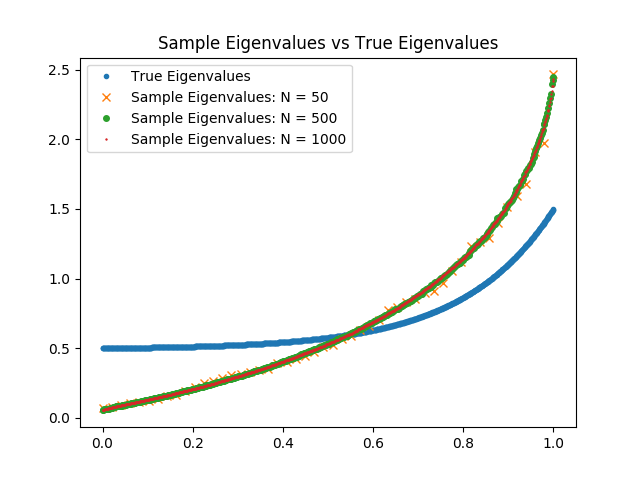
\includegraphics[width=5in]{eigs.png}
	\caption{
		Example of sample covariance eigenvalue spectrum for various $N$ and $y=2$.
		The true eigenvalue spectrum is given by $H_\gamma(\tau) = \frac{1 -
		e^{-\gamma(\tau - 1)}}{1 - e^{-\gamma}}$ with $\mathrm{supp}(H) = [1, 2]$.
		The true spectrum is approximated for some $N$ by $\tau_i = 1 - \frac1\gamma
		\log\left( 1 - x_i(1-e^{-\gamma}) \right)$ where $x_i = \frac{i - 1}{N - 1},\
		i = 1, \ldots, N$.
	}
	\label{fig:eigs}
\end{figure}


Define the sample covariance matrix as,
$$
	S_N = \frac1T X_N^T X_N
$$
and the e.s.d.\ of $S_N$ as
$$
	F_N(\lambda)
		 = \frac{1}{N}\sum_{i=1}^N \mathbbm{1}_{[\lambda_{i}, +\infty)}(\lambda)
$$
where $\lambda_{1}, \ldots, \lambda_N$ is the system of eigenvalues.  It is not
assumed that $F_N$ has a limit or what it is.  That's where the Marchenko-Pastur
theorem comes in.


\section{Main Marchenko-Pastur Result}


The main result of RMT and Marchenko-Pastur (MP) is convergence of $F_N$ to a
limit law $F$ almost surely. The result is not direct but instead states
convergence in terms of the \emph{Stieltjes transform} of $F_N$ and $F$.

The Stieltjes transform of a nondecreasing function $G$ is,
$$
	m_G(z) = \int_{-\infty}^\infty \frac{dG(x)}{x - z}
$$
where $z \in \mathbb{C}^+ = \left\{ z \in \mathbb{C}: \mathrm{Im}(z) >
0\right\}$.

For an empirical distribution like $F_N$, this is,
$$
	m_{F_N}(z)
		 = \frac1T \sum_{i=1}^N \frac{1}{\lambda_{i} - z}
		 = \frac1T \Tr\left[(S_n - zI)^{-1}\right]
$$

The Marchenko-Pastur result is that $m_{F_N}(z) \rightarrow m_{F}(z)$ almost
surely for all $z \in \mathbb{C}^+$ and $m_{F}(z)$ is defined through the \emph
{Marchenko-Pastur equation},
$$
	m_F(z) = \int_{\mathrm{supp}(H)}
			 \frac{dH(\tau)}{\tau\left[1 - y^{-1} - y^{-1}z m_F(z) \right] - z}.
$$
In few cases\footnote{Perhaps only one?  This would be the case when all
eigenvalues are equal to a common value} can this equation be solved
analytically.  It can potentially be solved numerically for specified $H$ but
that is not really important.  Moreover, the limit $F$ would come from the
inversion of $m_F(z)$ given by,
$$
	F(b) - F(a) = \lim_{\eta \rightarrow0^+} 
			\frac1\pi \int_a^b \mathrm{Im}\left[ m_F(\xi + i\eta\right] d\xi
$$

Figure \ref{fig:eigs} shows the e.s.d.\ $F_N$ for various values of $N$.  It may
be difficult to see but for $N=1000$, the e.s.d.\ shows convergence to the limit
compared to $N=50$.

\subsection{A Generalization of M-P}

\cite{Ledoit2011Eigenvectors} show how you can generalization to functions like
$$
	\Omega^g_N(\lambda)
		 = \frac{1}{N}\sum_{i=1}^N \mathbbm{1}_{[\lambda_{i}, +\infty)}(\lambda)
		 			\sum_{j=1}^N |u_i^T v_j|^2 g(\tau_j)
$$
where
\begin{gather*}
	S_N = U\Lambda U^T, 
		\quad U = \begin{bmatrix} u_1 & \cdots & u_N \end{bmatrix}
		\quad \Lambda = \mathrm{Diag}(\lambda_1, \ldots, \lambda_N),\\
	\Sigma_N = V T V^T, 
		\quad V = \begin{bmatrix} v_1 & \cdots & v_N \end{bmatrix}
		\quad T = \mathrm{Diag}(\tau_1, \ldots, \tau_N)
\end{gather*}

The Stieltjes transform of $\Omega^g_N$ is given by,
\begin{align*}
	\Theta^g_N(z)
		& = \frac{1}{N}\sum_{i=1}^N \frac{1}{\lambda_i - z}
		  		\sum_{j=1}^N |u_i^T v_j|^2 g(\tau_j) \\
		& = \frac{1}{N}\Tr\left[(S_N - zI)^{-1} g(\Sigma_N)\right]
\end{align*}
where in an abuse of notation, $g(\Sigma_N)$ is considered as a spectral
function, ie. it applies $g$ to the eigenvalues of $\Sigma_N$.

The way to see how the Trace operator relates, you just do some simple linear
algebra:
\begin{align*}
	\Tr\left[(S_N - zI)^{-1} g(\Sigma_N)\right]
		& = \Tr\left[( U\Lambda U^T - zI)^{-1} V g(T) V^T \right] \\
		& = \Tr\left[U^T(\Lambda - zI)^{-1} UV g(T) V^T \right] \\
		& = \Tr\left[(\Lambda - zI)^{-1} (UV) g(T) (UV)^T \right]
\end{align*}
where expanding out the last term gives $\Theta^g_N(z)$.  Furthermore, if you
take $g \equiv 1$, then you get back $F_N$ and $m_{F_N}$.

The generalized result for $\Omega^g_N(\lambda)$ and $\Theta^g_N(z)$ is $\Theta^g_N(z)$
converges a.s.\ to $\Theta^g(z)$ for all $z \in \mathbb{C}^+$ where $\Theta^g(z)$ 
is given by,
$$
	\Theta^g(z) = \int_{\mathrm{supp}(H)}
			 \frac{g(\tau)dH(\tau)}{\tau\left[1 - y^{-1} - y^{-1}z m_F(z) \right] - z}.
$$

Note how the integration kernel in the denominator stays the same and the result
only differs in our weighting scheme $g(\tau)$.

\subsection{Optimal Shrinkage}

\subsubsection{Frobenius Loss}\label{sec:fro_loss}

If we consider the class of estimators
$$
	\hat{\Sigma}_N = U D U^T
$$
where $U$ are the eigenvectors of the sample covariance matrix, then we can try
to minimize Frobenius error via,
$$
	\min_D \| UDU^T - \Sigma_N\|_F^2
$$
The optimal eigenvalues are
\begin{align}\label{eq:fro_oracle}
	D^* = \mathrm{Diag}(\tilde{d}_1, \ldots, \tilde{d}_N)
		  = \mathrm{Diag}(u_1^T \Sigma_N u_1, \ldots, u_N^T\Sigma_N u_N)
\end{align}

From before, if we take $\Omega^g_N(\lambda)$ and $\Theta^g_N(z)$ for $g(\tau) =
\tau$, then if we define,
$$
	\Delta_N(\lambda)
		 = \frac1N \sum_{i=1}^N 
		 			\tilde{d}_i \mathbbm{1}_{[\lambda_i, \infty)}(\lambda)
		 = \Omega^g_N(\lambda)
$$
then based on previous stated result about the convergence of $\Theta^g_N(z)$,
\cite{Ledoit2011Eigenvectors} show through verifying with calculus that
$\Delta_N(\lambda) \rightarrow \Delta(\lambda)$ almost surely for all $\lambda
\ne 0$ and
$$
	\Delta(\lambda) = \Omega^g(\lambda) = \int_{-\infty}^\lambda \delta(x)dF(x)
$$
where 
$$
	\delta(\lambda) = 
		\begin{cases}
			\frac{\lambda}{|1 - y^{-1} - y^{-1}\lambda m_F(\lambda)|^2} & \lambda > 0,\\
			% \frac{y}{(1 - y)m_F(0)} & \lambda = 0,\\
			0 & \text{otherwise.}
		\end{cases}
$$


The summary of this is that while the oracle estimates that are optimal,
$\tilde{d}_i = u_i^T \Sigma_N u_i$, are completely infeasible, we use
$\delta(\lambda_i)$ as the consistent estimate for $\tilde{d}_i$. This is seen
by considering,
$$
	\tilde{d}_i = \lim_{\epsilon \rightarrow 0^+} 
		\frac{\Delta_N(\lambda_i + \epsilon) - \Delta_N(\lambda_i - \epsilon)}
			{F_N(\lambda_i + \epsilon) - F_N(\lambda_i - \epsilon)}
		\approx \delta(\lambda_i)
$$
where the approximation comes from the asymptotic theory.  Now, it remains to
actually estimate $m_F(z)$ and thus produce a consistent estimate of the
shrinkage function but this has in fact been done in \cite{Ledoit2015Spectrum}.


\subsubsection{Out-of-Sample Variance Loss}\label{sec:oos_var_loss}

The goal here is to minimize
$$
	\mathcal{L}(\hat{\Sigma}_N, \Sigma_N, m)
		:= \hat{w}^T \Sigma_N \hat{w}
		 = m^Tm \times \frac
		 	{m^T \hat{\Sigma}_N^{-1} \Sigma_N \hat{\Sigma}_N^{-1} m}
		 	{\left(m^T \hat{\Sigma}_N^{-1} m\right)^2}
$$
for some rotation-equivariant estimator $\hat{\Sigma}_N$ given by 
$$
	\hat{\Sigma}_N = U D U^T
$$
where $D = \mathrm{Diag}(\hat{\rho}(\lambda_1), \ldots,
\hat{\rho}(\lambda_N))$ and $U$ are the eigenvectors of $S_N$.  Here $\hat{w}$
is a scaled form of the long-short maximum Sharpe ratio portfolio,
$$
	\hat{w} 
		= \frac{\sqrt{ m^Tm }}{m^T \hat{\Sigma}_N^{-1} m} \times \hat{\Sigma}_N^{-1} m.
$$
where $m$ is the \emph{return predictive signal} aka expected return and is
distributed independently of $S_N$ and its distribution is rotation invariant.
The scaling $\sqrt{ m^Tm }$ was chosen so that the portfolio weights are
invariant to $m$.

From Lemma 1 in \cite{Ledoit2011Eigenvectors} based on the properties of $m$,
$$
	\frac1N m^T \hat{\Sigma}_N^{-1} m 
		- \frac1N \Tr(\hat{\Sigma}_N^{-1}) \rightarrow 0,
$$
almost surely so that they converge together to,
$$
	\int \frac{1}{\hat{\rho}(\lambda)}dF(\lambda)
$$

A similar line of reasoning shows that 
$$
	\frac1N m^T \hat{\Sigma}_N^{-1} \Sigma_N \hat{\Sigma}_N^{-1} m
		- \frac1N \Tr(\hat{\Sigma}_N^{-1} \Sigma_N \hat{\Sigma}_N^{-1})
		\rightarrow 0
$$
almost surely so that they converge together.  To what becomes evident by
looking at the theorems for the generalization of the M-P result.  Namely,
$$
	\frac1N \Tr(\hat{\Sigma}_N^{-1} \Sigma_N \hat{\Sigma}_N^{-1})
		 = \frac1N \Tr(U^T \Sigma_N U D^{-2})
		 = \frac1N \sum_{i=1}^N \frac{u_i^T \Sigma_N u_i}{\hat{\rho}(\lambda_i)^2}
$$
But this is basically the same as $\Delta_N$ from the previous section, so it
turns out that the limit is,
$$
	\int \frac{\delta(\lambda)}{\hat{\rho}(\lambda)^2}dF(\lambda)
$$

These two limit results show that,
$$
	\mathcal{L}(\hat{\Sigma}_N, \Sigma_N, m)
		 \rightarrow \frac
		 		{\int \frac{\delta(\lambda)}{\hat{\rho}(\lambda)^2}dF(\lambda)}
		 		{\left( \int \frac{1}{\hat{\rho}(\lambda)}dF(\lambda) \right)^2}.
$$

Differentiation with respect to $\hat{\rho}(\lambda)$\footnote{I tried replicating this
result in the Goldilocks paper but I can't get it right} yields the result that
the first order condition is satified if and only if,
$$
	\frac{\hat{\rho}(\lambda)}{\delta(\lambda)} = c
$$
where $c$ is an arbitrary constant.  Choosing the constant equal to 1 satisfies
some consistency results with regards to Traces of the estimator and the
population covariance.

The upshot here is that even for this new loss function, the shrinkage is
actually the same as the one for the Frobenius norm.

\subsection{Cross-Validation for Optimal Shrinkage}

The optimal shrinkage is $\delta(\lambda)$ and thus is the quantity of interest.

\subsubsection{Leave-One-Out CV}\label{sec:loo}

Based on the suggestion of a referee, in Remark 5.2 of
\cite{Ledoit2012Nonlinear}, a cross-validated estimator is proposed.  It is
given here. Let $\left(\lambda_1^{(k)}, \ldots, \lambda_N^{(k)}\right)$ and
$\left(u_1^{(k)}, \ldots, u_N^{(k)}\right)$ denote a system of eigenvalues and
eigenvectors of the sample covariance matrix computed from all the observed
data, except for the $k$-th observation $x_k$.

From Sections \ref{sec:fro_loss} and \ref{sec:oos_var_loss}, the quantity to
compute is,
$$
	\tilde{d}_i= u_i^T \Sigma_N u_i,
$$
which leads to the cross-validation approximation,
$$
	\tilde{d}_i \approx \rho^{cv}(\lambda_i) 
		\equiv \frac1T \sum_{k=1}^T ({u_i^{(k)}}^T x_k)^2
$$

The motivation comes from the fact that,
$$
	({u_i^{(k)}}^T x_k)^2 = {u_i^{(k)}}^T x_k x_k^T u_i^{(k)} 
$$
where $x_k$ is independent of $u_i^{(k)}$ and $\mathbb{E}\left[x_k x_k^T\right]
= \Sigma_N$. Therefore,
$$
	\mathbb{E}\left[\rho^{cv}(\lambda_i)\right]
		 = \mathbb{E}\left[{u_i^{(k)}}^T x_k x_k^T u_i^{(k)}\right]
		 = \mathbb{E}\left[{u_i^{(k)}}^T \Sigma_N u_i^{(k)}\right]
$$

The full algorithm is given by Algorithm \ref{alg:nls_loo}.

\begin{algorithm}
	\caption{Leave-One-Out Cross Validation for Non-Linear Shrinkage}
	\label{alg:nls_loo}
	\begin{algorithmic}[1]
	\Require $X = [x_1, \ldots, x_T]^T \in \mathbb{R}^{T\times N}$
	\Require $\Sigma_N = \mathrm{Cov}(X)$
	\Procedure{LOO-CV}{$X$}

		\State $S \gets \frac1T X^T X$
		\State 
				$U \gets [u_1, \ldots, u_N] \in \mathbb{R}^{N\times N}$,
				\quad $\Lambda \gets \mathrm{Diag}(\lambda_1, \ldots, \lambda_N)$,
				\quad \mbox{s.t.}\quad $S = U \Lambda {U}^T$

		\State $\tilde{d} \gets [0, \ldots, 0]^T \in \mathbb{R}^{N}$
		\While{$k\le T$}
			\State $X_{-k} \gets [x_1, \ldots, x_{k-1}, x_{k+1}, \ldots, x_T]^T$
			\State $S^{(k)} \gets \frac{1}{T-1} X_{-k}^T X_{-k} $
			\State 
				$U^{(k)} \gets [u^{(k)}_1, \ldots, u^{(k)}_N] \in \mathbb{R}^{N\times N}$,
				\quad $\Lambda^{(k)} 
					\gets \mathrm{Diag}(\lambda^{(k)}_1, \ldots, \lambda^{(k)}_N)$,
				\quad \mbox{s.t.}\quad $S^{(k)} = U^{(k)} \Lambda^{(k)} {U^{(k)}}^T$
			\State $\tilde{d}_i \gets \tilde{d}_i 
				+ \frac1T ({U^{(k)}}^T x_k)_i^2, \quad i = 1, \ldots, N$
			\State $k \gets k+1$
		\EndWhile

		\State $\hat{\Sigma}_N \gets UDU^T, \quad 
			\mbox{where}\quad D = \mathrm{Diag}(\tilde{d}_1, \ldots, \tilde{d}_N)$

		\State \textbf{return} $\hat{\Sigma}_N$ 
				\Comment{The LOO-CV non-linear shrinkage estimator for $\Sigma_N$.}
	\EndProcedure
	\end{algorithmic}
\end{algorithm}



\subsubsection{K-Fold CV}\label{sec:kcv}

The standard LOO cross-validation estimator in the previous section is known to
have poor properties, as discussed in \cite{Bartz2016CrossValidation}.  One
possible fix is to use $K$-fold sampling of the data to produce an estimate,
$$
	\rho^{kcv}(\lambda_i) 
		\equiv \frac1K \sum_{k=1}^K {u_i^{(k)}}^T X_k X_k^T u_i^{(k)}
$$
where $X_k$ contains the observations from the $k$-th fold and $u_i^{(k)}$ is
the $i$-th eigenvector of the sample covariance matrix computed on the data with
the $k$-th fold removed.


\begin{algorithm}
	\caption{$K$-Fold Cross Validation for Non-Linear Shrinkage}
	\label{alg:nls_kcv}
	\begin{algorithmic}[1]
	\Require $X = [x_1, \ldots, x_T]^T \in \mathbb{R}^{T\times N}$
	\Require $\Sigma_N = \mathrm{Cov}(X)$
	\Require $K \in \mathbb{Z}, \quad K > 1$
	\Procedure{$K$-Fold-CV}{$X$}

		\State $S \gets \frac1T X^T X$
		\State 
				$U \gets [u_1, \ldots, u_N] \in \mathbb{R}^{N\times N}$,
				\quad $\Lambda \gets \mathrm{Diag}(\lambda_1, \ldots, \lambda_N)$,
				\quad \mbox{s.t.}\quad $S = U \Lambda {U}^T$

		\State $m \gets T / K$
		\State $\mathcal{K} \gets \{(1, \ldots m), \ldots, (T-m+1, \ldots, T)\}$

		\State $\tilde{d} \gets [0, \ldots, 0]^T \in \mathbb{R}^{N}$
		\State $k \gets 1$
		\While{$k\le K$}
			\State $X_{-k} \gets [x_{j_1}, \ldots, x_{j_{(T-m)}}]^T \in \mathbb{R}^{(T-m)\times N}, 
				\quad j_i \notin \mathcal{K}_k$
			\State $X_{k} \gets [x_{\ell_1}, \ldots, x_{\ell_m}]^T \in \mathbb{R}^{m\times N}, 
				\quad \ell_i \in \mathcal{K}_k$
			\State $S^{(k)} \gets \frac{1}{T-m} X_{-k}^T X_{-k} $

			\State 
				$U^{(k)} \gets [u^{(k)}_1, \ldots, u^{(k)}_N] \in \mathbb{R}^{N\times N}$,
				\quad $\Lambda^{(k)} 
					\gets \mathrm{Diag}(\lambda^{(k)}_1, \ldots, \lambda^{(k)}_N)$,
				\quad \mbox{s.t.}\quad $S^{(k)} = U^{(k)} \Lambda^{(k)} {U^{(k)}}^T$


			\State $\tilde{d}_i \gets \tilde{d}_i 
				+ \frac1T {u^{(k)}_i}^T (\frac1m X_{k}^T X_{k}) u^{(k)}_i 
				\quad i = 1, \ldots, N$
			\State $k \gets k+1$
		\EndWhile

		\State $\hat{\Sigma}_N \gets UDU^T, \quad 
			\mbox{where}\quad D = \mathrm{Diag}(\tilde{d}_1, \ldots, \tilde{d}_N)$

		\State \textbf{return} $\hat{\Sigma}_N$ 
				\Comment{The $K$-Fold-CV non-linear shrinkage estimator for $\Sigma_N$.}
	\EndProcedure
	\end{algorithmic}
\end{algorithm}

\subsubsection{Isotonic-Leave-One-Out CV}\label{sec:icv}

Another easy and well-behaved fix is to apply isotonic regression to produce an
improved estimator $\rho^{icv}(\lambda_i)$.   This is given by the solution to
the optimization problem,
\begin{equation*}
  \begin{aligned}
    & \underset{a_1, \ldots, a_N}{\text{minimize}}
    & & \sum_{i=1}^N (a_i - \rho^{cv}(\lambda_i))^2 \\
    & \text{subject to}
    & & a_i > a_{i+1},\\
    & & & \sum_{i=1}^N a_i = \sum_{i=1}^N \rho^{cv}(\lambda_i).
  \end{aligned}
\end{equation*}

\subsubsection{Isotonic-K-Fold CV}\label{sec:ikcv}

The isotonic regression can also be applied to the $K$-fold CV estimator that
will be called $\rho^{ikcv}(\lambda_i)$.

\subsubsection{Performance}

\cite{Bartz2016CrossValidation} shows that $\rho^{cv}(\lambda_i)$ is terrible as
an estimator.  The main issue is instability in the eigenvalues/eigenvectors
when dropping a single observation.  This is most simply mitigated by using
$\rho^{kcv}(\lambda_i)$, which shows huge improvement in Figure \ref{fig:cv}.
Applying isotonic regression, whether to the $\rho^{cv}(\lambda_i)$ or
$\rho^{kcv}(\lambda_i)$ gives the best results.


	\begin{figure}[htbp]
		\centering
		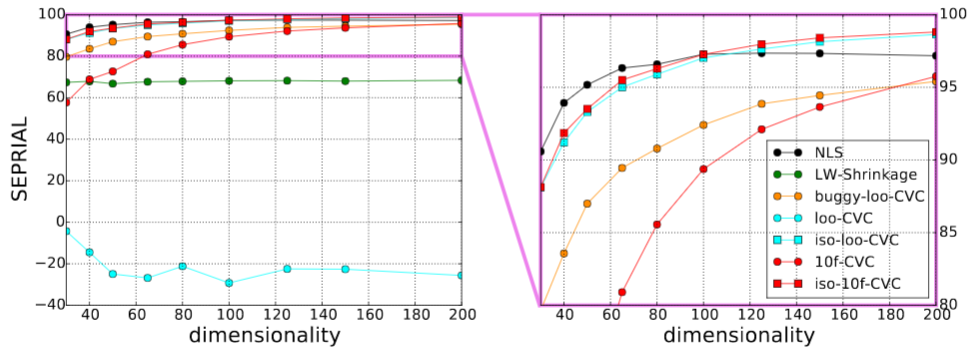
\includegraphics[width=6in]{cv.png}
		\caption{
			From \cite{Bartz2016CrossValidation}.  Estimation error of cross-
			validated covariance estimators from \cite{Bartz2016CrossValidation}.
			Averaged over 50 repetitions.  \emph{NLS} refers to the LW optimal
			shrinkage. \emph{LW-Shrinkage} refers to the linear shrinkage of
			\cite{Ledoit2004WellConditioned}. \emph{buggy-loo-CVC} refers to an
			incorrectly implemented leave-one-out cross-validated estimator that
			appears in \cite{Ledoit2012Nonlinear}. \emph{loo-CVC} refers to the
			correctly implemented leave-one-out cross-validated estimator proposed in
			\cite{Ledoit2012Nonlinear} and described in Section \ref{sec:loo}. \emph
			{iso-loo-CVC} refers to the isotonic version of the leave-one-out cross-
			validated estimator described in \ref{sec:icv}.  \emph {10f-CVC} refers to
			the 10-fold cross-validated estimator described in \ref{sec:kcv}.  And
			\emph{iso-10f-CVC} refers to the 10-fold, isotonic cross-validated
			estimator described in \ref{sec:ikcv}. }
		\label{fig:cv}
	\end{figure}


\section{Optimal Shrinkage for Unbiased Variance Ratios}



There are a few problems with the above methodologies that we have run into (and
need to solidly verify numerically):
\begin{enumerate}
	\item The above method produces a covariance matrix that will minimize out-of-
	sample variance for any portfolio that is colinear with that tangency
	portfolio.  In that sense, it is optimal.  But what about another portfolio?
	What about the minimum variance (global or long-only) portfolio?  Is it still
	the correct shrinkage if you are interested in computing the minimum variance
	portfolio?

	\item Numerical results (need to verify again) indicate the variance ratios
	for minimum variance portfolio computed from the optimal non-linear shrunk
	covariance matrix are suboptimal.  That is, they are not unbiased around 1.  
  As we will see, the optimal non-linear shrunk covariance matrix should produce
  good variance ratios for the tangency portfolios (need to verify numerically).


\end{enumerate}

Consider the loss function,
$$
	\mathcal{R}(\hat{\Sigma}_N, \Sigma_N, \hat{w}_N)
		:= \left(
			1 - \frac{\hat{w}_N^T \hat{\Sigma}_N \hat{w}_N} {\hat{w}_N^T \Sigma_N \hat{w}_N}
			\right)^2
$$
% $$
% 	\mathcal{R}(\hat{\Sigma}_N, \Sigma_N, \hat{w}_N)
% 		:= \left(
% 			\hat{w}_N^T \Sigma_N \hat{w}_N - \hat{w}_N^T \hat{\Sigma}_N \hat{w}_N 
% 			\right)^2
% $$
where $\hat{w}_N$ is some portfolio rule dependent on the covariance matrix
and $\hat{\Sigma}_N$ is an estimator.

\subsection{Maximum Sharpe Portfolio}

\begin{thm}[Oracle Shrinkage for Variance Ratio of Maximum Sharpe Ratio
	Portfolio] Under the same setup as Theorem 4.1 of \cite{Ledoit2017Nonlinear},
	the same oracle estimator of the covariance matrix that that minimizes out-of-
	sample variance also minimizes the almost sure limit of the loss function
	$\mathcal{R}(\hat{\Sigma}_N, \Sigma_N, \hat{w}_N)$.
\end{thm}

{\bf Sketch:}

If we consider the same maximum Sharpe ratio portfolios as before, then,
$$
	\mathcal{R}(\hat{\Sigma}_N, \Sigma_N, \hat{w}_N)
		:= \left(
				1 - \frac{m^T \hat{\Sigma}_N^{-1} \Sigma_N \hat{\Sigma}_N^{-1} m} 
								 {m^T \hat{\Sigma}_N^{-1} m}
			\right)^2.
$$

% $$
% 	\mathcal{R}(\hat{\Sigma}_N, \Sigma_N, \hat{w}_N)
% 		= \left(
% 				m^T \hat{\Sigma}_N^{-1} \Sigma_N \hat{\Sigma}_N^{-1} m
% 				 - m^T \hat{\Sigma}_N^{-1} m
% 			\right)^2.
% $$

From the same theory as above,
$$
	\mathcal{R}(\hat{\Sigma}_N, \Sigma_N, \hat{w}_N)
	 	\rightarrow 
		 	\left(
				1 - \frac{\int \frac{\delta(\lambda)}{\hat{\rho}(\lambda)^2}dF(\lambda)}
				 				 {\int \frac{1}{\hat{\rho}(\lambda)}dF(\lambda)}
			\right)^2,
$$
which is minimized and equal to 0 if $\hat{\rho}(\lambda) = \delta(\lambda).$
Moreover, this indicates the optimal non-linear shrinkage estimator should
provide good variance forecasting for the maximum Sharpe ratio portfolio.



\subsection{Global Minimum Variance Portfolio}

Now we consider the global minimum variance portfolio,
$$
	\hat{w}_N = \frac{\hat{\Sigma}_N^{-1}\mathbbm{1}}
						{\mathbbm{1}^T\hat{\Sigma}_N^{-1}\mathbbm{1}}.
$$

The loss function is given by,
$$
	\mathcal{R}(\hat{\Sigma}_N, \Sigma_N, \hat{w}_N)
		= \left(
				1 - 
					\frac{\mathbbm{1}^T \hat{\Sigma}_N^{-1} \Sigma_N \hat{\Sigma}_N^{-1} \mathbbm{1}}
						   {\mathbbm{1}^T \hat{\Sigma}_N^{-1} \mathbbm{1}}
			\right)^2.
$$
% $$
% 	\mathcal{R}(\hat{\Sigma}_N, \Sigma_N, \hat{w}_N)
% 		= \left(
% 				\mathbbm{1}^T \hat{\Sigma}_N^{-1} \Sigma_N \hat{\Sigma}_N^{-1} \mathbbm{1}
% 					- \mathbbm{1}^T \hat{\Sigma}_N^{-1} \mathbbm{1}
% 			\right)^2.
% $$

Letting $\alpha = U^T \mathbbm{1}$, the above loss can be written as,
$$
	\mathcal{R}(\hat{\Sigma}_N, \Sigma_N, \hat{w}_N)
		= \left(
				1 - \frac{\alpha^T D^{-1} U^T\Sigma_N U D^{-1} \alpha}
						   {\alpha^T D^{-1} \alpha}
			\right)^2.
$$
% $$
% 	\mathcal{R}(\hat{\Sigma}_N, \Sigma_N, \hat{w}_N)
% 		= \left(
% 			\alpha^T D^{-1} U^T\Sigma_N U D^{-1} \alpha
% 				 - \alpha^T D^{-1} \alpha
% 			\right)^2.
% $$

\subsubsection{Oracle Optimal Shrinkage}

\begin{thm}[Oracle Shrinkage for Variance Ratio of Minimum Variance Portfolio]
	Let $X \in \mathbb{R}^{T \times N}$ denote $T$ i.i.d.\ draws from an
	$N$-dimensional distribution with covariance $\Sigma_N$.  Define the sample
	covariance matrix as $S = \frac1T X^T X$ with eigendecomposition $S = U\Delta
	U^T$.

	Let the class of rotation invariant covariance estimators be defined by,
	$$
		\hat{\Sigma}_N = U D U^T
	$$
	where $D= \mathrm{Diag}({d}_1, \ldots, {d}_N)$ are the chosen eigenvalues for
	the estimator.

	Finally, define the plug-in estimator for global minimum variance portfolio
	as
	$$
		\hat{w}_N = \frac{\hat{\Sigma}_N^{-1}\mathbbm{1}}
						{\mathbbm{1}^T\hat{\Sigma}_N^{-1}\mathbbm{1}}.
	$$

	The optimal finite sample oracle shrinkage estimator $\hat{\Sigma}^*_N = U D^*
	U^T$ with respect to the loss function $\mathcal{R}(\hat{\Sigma}_N, \Sigma_N,
	\hat{w}_N)$ is given by $D^*_{ii} = d^*_i = 1 / z_i$ where $z \in
	\mathbb{R}^N$ is the solution to the linear system,
	$$
		C A z = \alpha.
	$$
	for $C = U^T\Sigma_N U$, $\alpha = U^T \mathbbm{1}$, and $A =
	\mathrm{Diag}(\alpha_1, \ldots, \alpha_N)$.

	This estimator also minimizes out-of-sample variance,
	$$
		\mathcal{L}(\hat{\Sigma}_N, \Sigma_N, \hat{w}_N)
			 = \hat{w}_N^T \Sigma_N \hat{w}_N
			 = \frac
  				{\mathbbm{1}^T \hat{\Sigma}_N^{-1} \Sigma_N  \hat{\Sigma}_N^{-1} \mathbbm{1}}
  				{\left( \mathbbm{1}^T \hat{\Sigma}_N^{-1} \mathbbm{1}\right)^2}
	$$
\end{thm}

{\bf Sketch:}

From the preceding section, we can write,
$$
	\alpha^T D^{-1} \alpha 
		 = \Tr(D^{-1} \alpha \alpha^T)
		 = \sum_{i=1}^N \frac{\alpha_i^2}{{d}_i}
$$
and,
$$
	\alpha^T D^{-1} U^T\Sigma_N U D^{-1} \alpha
		 = \Tr(D^{-1} U^T\Sigma_N U D^{-1} \alpha \alpha^T)
		 = \sum_{i=1}^N \frac{\alpha_i}{{d}_i} 
		 			\sum_{j=1}^N \frac{C_{ij}\alpha_j}{{d}_j}
$$
where $C = U^T\Sigma_N U$ and $C_{ij} = u_i^T \Sigma_N u_j$.

If we can choose ${d}_i$ to equate $\alpha_i$ and
$\frac{C_{ji}\alpha_j}{{d}_j}$, then the loss function
$\mathcal{R}$ will be minimized and equal to 0.  This can be achieved by solving
a linear system.

Let,
$$
	A = \mathrm{Diag}(\alpha_1, \ldots, \alpha_N)
$$

Then ${d}_i = 1 / z_i$ where $z \in \mathbb{R}^N$ is the solution to,
$$
	C A z = \alpha.
$$
This gives
$$
	z = A^{-1} U^T \Sigma_N^{-1} U \alpha
		 = A^{-1} U^T \Sigma_N^{-1} \mathbbm{1}
$$

It turns out this estimator also minimizes out-of-sample variance for the global
minimum variance portfolio.  

The out-of-sample variance simplifies to,
$$
  \mathcal{L}(\hat{\Sigma}_N, \Sigma_N, \hat{w}_N) = \frac
  	{\alpha^T D^{-1} U^T \Sigma_N U D^{-1} \alpha}
  	{\left( \alpha^T D^{-1} \alpha\right)^2}
$$

Expanding terms as before and differentiating with respect to the $i$-th entry
in $D$ gives,
$$
  \frac{\partial\mathcal{L}}{\partial d_i} = -2 \frac
  	{ \frac{\alpha_i}{d_i^2} \sum_{j=1}^N \frac{C_{ij}\alpha_j}{d_j} }{ Q_2^2 }
    + 2\frac{ Q_1 }{ Q_2^3 } \frac{\alpha_i^2}{d_i^2}
$$
where $Q_1 = \alpha^T D^{-1} U^T \Sigma_N U D^{-1} \alpha$ and $Q_2 = \alpha^T
D^{-1} \alpha$.

The first-order condition $0 = \frac{\partial\mathcal{L}}{\partial d_i}$ reduces
to,
$$
  Q_2 \sum_{j=1}^N \frac{C_{ij}\alpha_j}{d_j}
   = Q_1 \alpha_i.
$$
If $d_i$ derived from the solution to $C A z = \alpha$, then $Q_2 = Q_1$ and the
first-order condition is satisfied.

To see this is a minimum, we rely on the chain-rule.  Let $F(w) = w^T \Sigma_N
w$ where $w$ is the plug-in estimator for global minimum variance portfolio
$\hat{w}_N$ and is therefore a function of $D$.

By the chain rule,
$$
	\nabla_D^2 F(w)
		 = \nabla_D^T w \cdot \nabla_w^2 F(w) \cdot (\nabla_D^T w)^T
		 	+ \nabla_D^2 w \cdot \nabla_w F(w)
$$
where,
\begin{gather*}
	(\nabla_D^2 F(w))_{ij} = \frac{\partial^2 F(w)}
																{\partial d_i \partial d_j},\\
	(\nabla_w F(w)_{i} = \frac{\partial F(w)}{\partial w_i},\\	
	(\nabla_w^2 F(w))_{ij} = \frac{\partial^2 F(w)}
																{\partial w_i \partial w_j},\\									
	(\nabla_D^T w)_{ij} = \frac{\partial w_i}{\partial d_j},\\													
	(\nabla_D^2 w)_{ijk} = \frac{\partial^2 w_i}
																{\partial d_j\partial d_k}.
\end{gather*}

The first-order condition means $\nabla_w F(w) = 0$ and thus since $\nabla_w^2
F(w) = 2\Sigma_N \succ 0$, $\nabla_D^2 F(w) \succ 0$.  This verifies that the
oracle estimator for $D^*$ minimizes out-of-sample variance.

\subsubsection{Asymptotically Optimal Shrinkage}

From the above, it may be possible to put $\mathcal{R}(\hat{\Sigma}_N,
\Sigma_N, \hat{w}_N)$ and the optimal oracle shrinkage in the RMT asymptotic
framework and derive the limiting results that would indicate how one should
choose $D$.  One possible work that may have related results is
\cite{Mestre2008Improved} which potentially derive the asymptotic results for
these kinds of functionals.  More needs to be done to study that work and check
if it fits the framework.

\subsubsection{Proposed Estimators}

The solution $z$ to the linear system,
$$
	C A z = \alpha,
$$
has a few issues with it.  First, despite being an oracle estimator like the
optimal values in \eqref{eq:fro_oracle}, the resulting values are very noisy.
The optimal values in \eqref{eq:fro_oracle} are also noisy so this is not a
problem exclusive to the new values.  Second, there are no guarantees on
positivity or monotonicty of the values $z$ or $d$.

The following are proposed estimators that seek to remedy these problems and
serve as \emph{bona fide} estimators.

\begin{enumerate}

\item \emph{Vanilla Leave-One-Out with Isotonic Regression}

The first proposed estimator is a simple cross-validation estimator using Leave-
One-Out cross-validation to generate multiple solutions to the above linear
system to stabilize estimates of the eigenvalues.

Let $C^{(k)} = {U^{(k)}}^T x_k x_k^T U^{(k)}$, $A^{(k)}$, and
$\alpha^{(k)}$ be the relevant quantities computed when leaving out the $k$-th
observation, $x_k$.

Then compute a set of intermediate values 
$$
	\bar{d}_i = \frac1T \sum_{k=1}^T \frac{1}{z_i^{(k)}}
$$
where $z^{(k)}$ is the solution to,
$$
	C^{(k)} A^{(k)} z^{(k)} = \alpha^{(k)}.
$$

Finally, the final estimator values are obtained following applying isotonic
regression such that,
$$
	\hat{d}^* = \mathrm{Isotonic}(\bar{d}).
$$

Variants could use a median computation instead of an averaging for computing
$\bar{d}$.  This is likely to be a better option because evidence suggests the
linear system produces widely ranging values.  Simple constraints like non-
negativity could also be used.

\item \emph{Vanilla $K$-Fold with Isotonic Regression}

A simple of the Leave-One-Out estimator, it uses $K$-Fold cross-validation
instead.

\item \emph{Joint Leave-One-Out with Isotonic Regression}

Averaging of the individual cross-validation values serves to denoise the raw
values to produce better performance before applying Isotonic regression.  The
solution $z$ could be obtained from solving the least squares problem,
$$
	\begin{array}{ll}
		\mbox{minimize} & \sum_{k=1}^T \| C^{(k)} A^{(k)} z - \alpha^{(k)} \|_2^2,
	\end{array}
$$
so that $\bar{d}_i = \frac{1}{z_i}$.  The final estimator is obtained via
Isotonic regression,
$$
	\hat{d}^* = \mathrm{Isotonic}(\bar{d}).
$$

\item \emph{Joint $K$-Fold with Isotonic Regression}

Again, similar to the above but with $K$-Fold cross-validation instead.

\item \emph{Nonlinear Leave-One-Out with Isotonic Regression}

Instead of solving in the changed variables $z_i = \frac{1}{d_i}$, one can
directly solve for $d_i = D_{ii}$ in,
$$
	\mathcal{R}(\hat{\Sigma}_N, \Sigma_N, \hat{w}_N)
		= \left(
				1 - \frac{\alpha^T D^{-1} U^T\Sigma_N U D^{-1} \alpha}
								 {\alpha^T D^{-1} \alpha}
			\right)^2.
$$

Of course, to make this a \emph{bona fide} estimator, we replace $U^T\Sigma_N U$
and $\alpha$ by $C^{(k)}$ and $\alpha^{(k)}$, respectively, to create the
objective function,
$$
	f(d; C, \alpha)
		 = \left( 
		 			1 - \frac{ \alpha^T D^{-1} C D^{-1} \alpha}{ \alpha^T D^{-1} \alpha }
			\right)^2,
$$
where $D = \mathrm{Diag}(d)$.  With $f(d; C, \alpha)$, we can employ several
different forms of estimator.

This basic estimator is computed similarly to the vanilla version.  Let
$d^{(k)}$ denote the solution to
$$
\begin{array}{ll}
	\mbox{minimize}   & f(d; C^{(k)}, \alpha^{(k)})
\end{array}
$$
where an optional non-negativity constraint $d \geq 0$ could be added.  Then
compute the set of intermediate values,
$$
	\bar{d} = \frac1T \sum_{k=1}^T d^{(k)},
$$
and finally apply Isotonic regression to get,
$$
	\hat{d}^* = \mathrm{Isotonic}(\bar{d}).
$$

As with the vanilla estimator, a variant could use a median computation instead
of an averaging for computing $\bar{d}$.

\item \emph{Nonlinear $K$-Fold with Isotonic Regression}

A similar estimator could be generated using $K$-fold cross-validation instead.

\item \emph{Joint Nonlinear Leave-One-Out with Isotonic Regression}

Optimal values $d$ could be obtained through joint minimization of $f(d;
C^{(k)}, \alpha^{(k)})$ for $k=1, \ldots, T$.  Intermediate values are obtained
from the optimization problem,
$$
\begin{array}{ll}
	\mbox{minimize}   & \sum_{k=1}^T f(d; C^{(k)}, \alpha^{(k)}).
\end{array}
$$
The final estimator is obtained after Isotonic regression,
$$
	\hat{d}^* = \mathrm{Isotonic}(\bar{d}).
$$

\item \emph{Joint Nonlinear $K$-Fold with Isotonic Regression}

Replace Leave-One-Out cross-validation above with $K$-fold cross-validation.

\item \emph{Joint Constrained Nonlinear Leave-One-Out}

Isotonic regression serves to create monotonicity in the estimated eigenvalues.
In the nonlinear optimization of $\sum_{k=1}^T f(d; C^{(k)}, \alpha^{(k)})$,
monotonicity constraints could be directly applied in the optimization problem.
Isotonic regression also seeks to preserve the trace of the estimated
eigenvalues so an additional trace constraint can be added.

For some target trace value $c$ and bounds $d_{\mbox{min}}$, $d_{\mbox{max}}$,
optimal values are obtained from the optimization problem,
$$
\begin{array}{ll}
	\mbox{minimize}   & \sum_{k=1}^T f(d; C^{(k)}, \alpha^{(k)}) \\
	\mbox{subject to} & G d \preceq 0, \\
										& \mathbbm{1}^T d = c,\\
										& d_{\mbox{min}} \leq d \leq d_{\mbox{max}},
\end{array}
$$
where $G \in \mathbb{R}^{(N-1)\times N}$ is a differencing matrix to ensure
monotonicity.

Variants could remove the trace constraint or either or both of the bounds.


Practical considerations for solving the optimization problem:

\begin{itemize}
	\item Gradient: 

	\begin{align*}
	  \frac{\partial}{\partial d_i} f(d; C, \alpha)
	    = 2\left( 
	    	1 - \frac{ \alpha^T D^{-1} C D^{-1} \alpha }
	    					 { \alpha^T D^{-1} \alpha }
	    	\right)
	    % \times \\
	    	\left( 
	       - \frac{-2\alpha_i}{d_i^2}
	       	 \sum_{j=1}^N \frac{C_{ij}\alpha_j }{d_j}
	         \frac{ 1 }{ \alpha^T D^{-1} \alpha}
	      + \frac{ -\alpha_i^2 }{ d_i^2 }
	        \frac{ \alpha^T D^{-1} C D^{-1} \alpha }{ (\alpha^T D^{-1} \alpha)^2}
	    \right)
	\end{align*}
	
	\item Change of Variables: $G$ adds $N-1$ linear inequality constraints to the 
	problem.  Augmenting a final row in $G$ to preserve $d_N$ creates an
	invertible transformation. Changing to differences gives:
	\begin{gather*}
		y = Gd, 
		\quad g(y; C, \alpha) = f(G^{-1}y; C, \alpha), 
		\quad \nabla_z g(y; C, \alpha) = G^{-T} \nabla_d f(G^{-1}y; C, \alpha),
	\end{gather*}
	The new optimization problem is,
	$$
	\begin{array}{ll}
		\mbox{minimize}   & \sum_{k=1}^T g(y; C^{(k)}, \alpha^{(k)}) \\
		\mbox{subject to} & y \geq [0, \ldots, 0, d_{\mbox{min}}]^T, \\
											& v^T y = c,\\
											& d_{\mbox{max}} - \mathbbm{1}^T y \geq 0,
	\end{array}
	$$
	where $v = G^{-T} \mathbbm{1}$ and creates the modified trace constraint, and
	the final constraint represents the upper bound $d_1 \leq d_{\mbox{max}}$.

	In implementation, $G$, $G^{-1}$, and $G{-T}$ can be performed without
	constructing matrices when inside the objective function or when transforming
	the gradient.  As a constraint, general nonlinear optimization routines will
	require $G$ in matrix form as a Jacobian of the constraint function.

	\item Preconditioning: This is still an open issue but a further scaling is
	possible such that $z = Py$ where $P$ is a diagonal matrix.

\end{itemize}

\item \emph{Joint Constrained Nonlinear $K$-Fold}

Replace Leave-One-Out cross-validation above with $K$-fold cross-validation.

\end{enumerate}



% \subsubsection{Cross-Validation Estimate of Optimal Shrinkage}

% Since obtaining the oracle shrinkage solves a linear system and previous cross-
% validation approaches used a low-rank matrix like $x_k x_k^T$ as a substitute
% for $\Sigma_N$, it is not immediately clear how to deal with this.  One possible
% method would be to solve for $z$ in a least squares sense:
% $$
% 	\hat{z} = \argmin \sum_{k=1}^T 
% 		\left\| C^{(k)}A^{(k)}z - \alpha^{(k)} \right\|^2
% $$
% where $C^{(k)} = {U^{(k)}}^T x_k x_k^T U^{(k)}$, $A^{(k)}$, and
% $\alpha^{(k)}$ are the relevant quantities computed when leaving the $k$-th
% observation out.  This can also be written in matrix form as,
% $$
% 	\begin{bmatrix} 
% 		C^{(1)}A^{(1)} \\ 
% 		\vdots                      \\ 
% 		C^{(T)}A^{(T)}
% 	\end{bmatrix} 
% 	z = 
% 	\begin{bmatrix} 
% 		\alpha^{(1)} \\ 
% 		\vdots       \\ 
% 		\alpha^{(T)}
% 	\end{bmatrix}.
% $$

% The isotonic constraints could also be applied to this least squares problem.


% This can be expressed as the solution to a quadratic program given by,
% $$
% \mbox{minimize}\quad (1/2) z^T P z + q^T z
% $$
% where
% $$
% 	P = \sum_{k=1}^T A^{(k)} {C^{(k)}}^T C^{(k)} A^{(k)},
% 	\quad q = -\sum_{k=1}^T A^{(k)} {C^{(k)}}^T \alpha^{(k)}.
% $$
% Without the contraints, this reduces to solving the system $Pz = -q$.

% The isotonic constraints lead to the constrained quadratic program,
% $$
% \begin{array}{ll}
% 	\mbox{minimize}   & (1/2) z^T P z + q^T z \\
% 	\mbox{subject to} & G z \preceq 0
% \end{array}
% $$
% where $G_{kk} = -1$, $G_{k,k+1} = 1$, and all other entries are 0.


\section{To Address}

\subsection{Metrics}

\begin{itemize}
	\item Out-of-Sample Variance
	\item Variance forecast
	\item Bias statistics: $r_w / (w\Sigma w)^{1/2}$
\end{itemize}

\subsection{Portfolios}

\begin{itemize}
	\item Global minimum variance
	\item Long-only minimum variance
	\item Equally weighted
	\item Maximum Sharpe Ratio
	\item Concentrated
\end{itemize}

\subsection{Models}

\begin{itemize}
	\item Covariances: simple factor, broad-narrow factor, identity, known $H$ with random $U$ or identity $U$
	\item Returns: equivariant
\end{itemize}


\subsection{Questions to Address}

\begin{itemize}
	\item What is the baseline performance of the classical sample covariance estimator?
	
	\item Does long-only outperform out-of-sample var vs global min var?

	\item When substituting in true eigenvectors and/or true eigenvalues, which is most important in fixing issues of estimation?  What does that tell us about covariance estimation?

	\item How does SLR improve when model is big factor model?  Where are its deficiencies?  With respect to which metrics or portfolios?
	
	\item How does non-linear shrinkage do?  Does the numerical verify the theory?  How is the var ratio for the Max Sharpe and min var portfolios?  Compare out of sample variance to portfolios along mean-variance frontier (true and estimated)
	
	\item Can we replicate the success/failure of non-linear shrinkage on the global min var and the long-only min var?
	
	\item For the oracle estimator for best var ratio performance: what portfolio does that give? Where does it fall on mean-variance frontier (true or estimated)?  Does it give unbiased var ratio? Does it give good var performance too despite being designed for var ratio?
	
	\item Does the cross-validated optimal var ratio estimator work?
\end{itemize}






% Alternatively, a cross-validation approach could be used.  A naive leave-one-out
% cross-validation estimator for the loss function would be,
% $$
% 	\mathcal{R}^{cv}
% 		= \frac1T \sum_{k=1}^T 
% 			\left(
% 				1 - \frac{{\alpha^{(k)}}^T D^{-1} \alpha^{(k)}}
% 			{{\alpha^{(k)}}^T D^{-1} {U^{(k)}}^T x_k x_k^T U^{(k)} D^{-1} \alpha^{(k)}}
% 			\right)^2.
% $$
% A similar $K$-fold cross-validation estimate $\mathcal{R}^{kcv}$ could be used.  

% An optimal shrinkage $D$ could be found by minimizing $\mathcal{R}^{cv}$ or
% $\mathcal{R}^{kcv}$ with respect to $D$.  It is likely that constraints would
% need to be put on $D$.  Like in the isotonic regression case, an ordering
% constrain is likely required as well as a constraint on the sum.  While it is
% not clear immediately what the sum constraint should be, Proposition 4.1 of
% \cite{Ledoit2017Nonlinear} indicates that the optimal non-linear shrinkage for
% the Maximum Sharpe Ratio portfolios preserves trace asymptotically.  Thus, the
% sum constraint would make the sum of the diagonals of $D$ (ie. its trace) the
% same as the trace of the optimal maximum Sharpe ratio covariance estimator.

% A few issues still remain:
% \begin{itemize}
% 	\item Will $\mathcal{R}^{cv}$ or $\mathcal{R}^{kcv}$ be good estimates of the
% 	loss? Unlike before, the cross-validation estimator is not using a function
% 	linear in $x_k x_k^T$.  Will that be a problem in cross-validation producing a 
% 	good estimate?

% 	\item We need a gradient formula for $\mathcal{R}^{cv}$ for any non-linear 
% 	optimizer.  Also, will optimizing the cross-validation estimate pose any
% 	problems?
% \end{itemize}
% These issues may not be problems at all and we can verify them in simulation.

% \section{A Different Portfolio than Maximum Sharpe?}

% What if the goal instead was to minimize out-of-sample variance but for a
% different portfolio?  Or even to minimize error from a variance ratio of 1?

% Consider the loss,
% $$
% 	\mathcal{L}(\hat{\Sigma}_N, \Sigma_N, \hat{w}_N)
% 		:= \left(
% 			1 - \frac{\hat{w}_N^T \hat{\Sigma}_N \hat{w}_N} {\hat{w}_N^T \Sigma_N \hat{w}_N}
% 			\right)^2
% $$
% where $\hat{w}_N$ is some portfolio rule dependent on the covariance matrix, like
% the global minimum variance portfolio
% $$
% 	\hat{w}_N = \frac{\hat{\Sigma}_N^{-1}\mathbbm{1}}
% 						{\mathbbm{1}^T\hat{\Sigma}_N^{-1}\mathbbm{1}},
% $$
% of the long-only minimum variance portfolio from
% $$
% 	\hat{w}_N = \argmin_w w^T \hat{\Sigma}_N w, 
% 		\quad \text{s.t. } \mathbbm{1}^T w = 1, \quad w \geq 0. 
% $$

% Using the eigenvectors $U$, we can rotate the portfolio $\hat{w}_N$ to the space of
% eigenportfolios where,
% $$
% 	\hat{w}_N = U\hat{\alpha}_N,
% $$
% so that,
% $$
% 	\mathcal{L}(\hat{\Sigma}_N, \Sigma_N, \hat{w}_N) = 
% 		\left(
% 			1 - \frac{\hat{\alpha}_N^T D \hat{\alpha}_N}
% 				{\hat{\alpha}_N^T U^T \Sigma_N U \hat{\alpha}_N}
% 		\right)^2
% $$

% It is likely that $\hat{\alpha}_N$ would converge to its own distribution
% $G(\lambda)$ as $N$ goes to infinity.  Perhaps then we would have something like
% $$
% 	\frac1N \hat{\alpha}_N^T D \hat{\alpha}_N 
% 		\rightarrow \int g(\lambda)^2 \hat{\rho}(\lambda)dF(\lambda)
% $$
% where $G'(\lambda) = g(\lambda)$.

% What would we get for the other term?
% $$
% 	\frac1N\hat{\alpha}_N^T U^T \Sigma_N U \hat{\alpha}_N
% $$
% The previous section had it relatively easy because the term fit well as defined
% through a Trace and matched up with previous theorems.  This can still be
% written as a Trace as,
% $$
% 	\frac1N\hat{\alpha}_N^T U^T \Sigma_N U \hat{\alpha}_N
% 	 = \frac1N \Tr(\hat{\alpha}_N^T U^T \Sigma_N U \hat{\alpha}_N)
% 	 = \frac1N \Tr(U^T \Sigma_N U \hat{\alpha}_N\hat{\alpha}_N^T)
% 	 = \frac1N \sum_{i=1}^N \alpha_i \sum_{j=1}^N |u_i^T v_j|^2 \tau_j \alpha_j
% $$
% Nothing pops out immediately that indicates what this would converge to.

% If convergence could be established, then perhaps we could tailor the shrinkage
% rule $\hat{\rho}$ to account for the portfolio weightings.

% Lastly, just for completeness, if you stick in the same scaled maximum Sharpe
% ratio portfolio into this new loss, the same convergence results carryover (all
% the objects are the same, naturally), so we get,
% $$
% 	\mathcal{L}(\hat{\Sigma}_N, \Sigma_N, \hat{w}_N)
% 		\rightarrow \left(
% 				1 - \frac{\int \frac{1}{\hat{\rho}(\lambda)}dF(\lambda)} 
% 					{\int \frac{\delta(\lambda)}{\hat{\rho}(\lambda)^2}dF(\lambda)}
% 			\right)^2
% $$
% which is minimized and equal to 0 if
% $$
% 	\hat{\rho}(\lambda) = \delta(\lambda).
% $$
% So perhaps the maximum Sharpe ratio portfolio has good variance ratio
% forecasting and minimum variance needs different shrinkage.  And as a last
% thought on this, perhaps a cross-validation approach that has been mentioned in
% some of these works (though crude and inefficient) could at least show how the
% minimum variance shrinkage needs to be different than the maximum Sharpe
% shrinkage.




% \newpage

% \section{Figures}

% 	\begin{figure}[htbp]
% 		\centering
% 		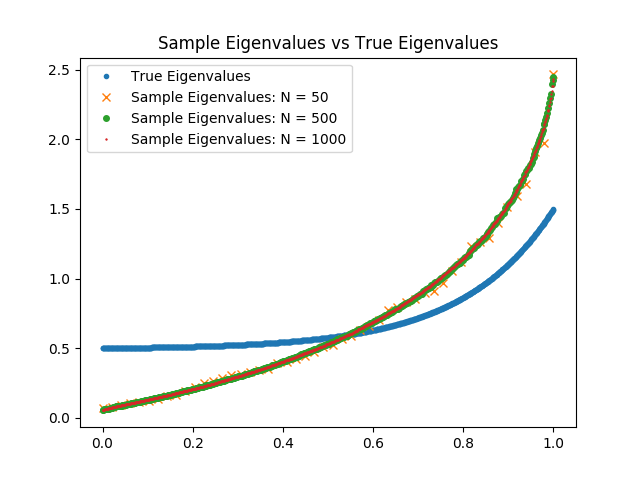
\includegraphics[width=5in]{eigs.png}
% 		\caption{}
% 		\label{fig:eigs}
% 	\end{figure}

\bibliographystyle{apalike}
\bibliography{Remote}

\end{document}